Sea  $\Omega' \subset \mathbb{R}^3$ el dominio de inter\'es, $t_f>0$ el tiempo final de la simulaci\'on,   $\vec v : [0,t_f]\times \Omega' \rightarrow  \mathbb{R}^3$ el campo de velocidad, y $p : [0,t_f] \times \Omega' \rightarrow \mathbb{R}$ el campo de presiones, de un fluido incompresible con densidad $\rho \in \mathbb{R}^+$, que escurre sobre un fondo (topograf\'ia - batimetr\'ia) de forma dada por $b:\Omega' \rightarrow \mathbb{R}$. Si se desprecian efectos disipativos y se consideran fuerzas de volumen $\vec f_b = (0,0,-g)^T$, con $g$ la aceleraci\'on de gravedad, las ecuaciones de Navier-Stokes son \cite{toro}
\begin{align}
  \begin{split}
    \nabla \cdot \vec v &= 0 \\
    \frac{\partial }{\partial t}\vec v + \nabla \cdot \vec v \otimes \vec v  &= -\frac{1}{\rho}\nabla p + \vec f_b    \\
    v_3|_{z=\eta	} &= \frac{\partial \eta}{\partial t}+(\vec v \cdot \nabla )\eta \\
    v_3|_{z=b} &= \frac{\partial b}{\partial t} + (\vec v \cdot \nabla )b \\    
    p|_{z = \eta} &= 0
  \end{split}  
  \label{NS-incompresible}
\end{align}

En particular, en una bah\'ia de interior $\Omega \subset \mathbb{R}^2$, con borde impermeable $\partial\Omega_h$ y linea nodal $\partial \Omega_g$ tales que $\partial \Omega = \partial \Omega_h \cup \partial \Omega_g$ , y bajo el supuesto que las ondas son suficientemente largas, de forma que las aceleraciones verticales no tienen influencia significtiva sobre el perfil de presiones hidrost\'atico, y por medio de integraci\'on vertical entre el fondo $b$ y la superficie libre $\eta$, las Ecuaciones No Lineales de Aguas Someras (Non-Linear Shallow water Equations, NSWE) son, 

\begin{align}  \begin{split}
\frac{\partial}{\partial t}\left(\eta\right)+\frac{\partial}{\partial x}\left(hu\right)+\frac{\partial}{\partial y}\left(hv\right) & =0  \text{       si } x \in \Omega\\
  \frac{\partial}{\partial t}\left(hu\right)+\frac{\partial}{\partial x}(hu^{2}+\frac{1}{2}gh^{2})+\frac{\partial}{\partial y}(huv) & =-gh\frac{\partial}{\partial x}b  \text{   si } x\in\Omega\\
  \frac{\partial}{\partial t}\left(hu\right)+\frac{\partial}{\partial x}(huv)+\frac{\partial}{\partial y}(hv^{2}+\frac{1}{2}gh^{2}) & =-gh\frac{\partial}{\partial y}b  \text{     si } x \in \Omega\\
  (hu,hv) \cdot \vec n &= 0  \text{ si    } x\in\partial \Omega_h \\
   \eta &= 0  \text{ si    } x \in \partial \Omega_g  
  \end{split}
  \label{eq:nswe_cart}
  \end{align}
donde, viendo la figura \ref{fig:vars}, $h:(t,x,y) \in [0,t_f] \times \Omega \to \eta(t,x,y)-b(x,y) \in \mathbb{R}^+$ es la altura de la columna de agua,  y $(u,v)$ las componentes de velocidad horizontal promediadas en la vertical, dadas por
 $$
  (u,v)=\frac{1}{h}\int_{b}^\eta (v_1,v_2)dz
 $$
  
  \begin{figure}
    \centering
    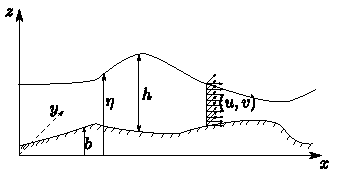
\includegraphics[width=10cm]{figs/variables.pdf}    
    \caption{ Vista esquem\'tica de ls varibles hidrodin\'amicas definidas para las Ecuaciones No Lineales de Aguas Someras (NSWE).}
    \label{fig:vars}
  \end{figure}

Las ecuaciones en \eqref{eq:nswe_cart}, forman un sistema hiperb\'olico de ecuaciones diferenciales parciales no lineales, que admite ondas de choque e interfaces seco-mojado, cuando $h$ tiende a $0$. Sin embargo, es posible obtener una linealizaci\'on del sistema \eqref{eq:nswe_cart} si se consideran peque\~nas perturbaciones a una masa de agua en reposo, es decir si
$$
	\eta=h_0+\eta' \hspace{.5cm} u=0+u',\hspace{.5cm} v = 0 + v'
$$
donde la notaci\'on $\square'$ indica peque\~nas perturbaciones sobre $\square$, y $h_0:\Omega\rightarrow \mathbb{R}$ representa la altura de la columna de agua, de forma que  \footnote{Aqu\'i el lector debe notar que este supuesto es equivalente a asumir que las ondas son de amplitud peque\~na.}
$$\left|\frac{\eta'(t,x,y)}{h_0(x,y)}\right|<<1$$
para cualquier $(t,x,y) \in [0,t_f]\times\Omega$. Bajo estos supuestos, se deducen las Ecuaciones Lineales de Aguas Someras (LSWE), dadas por
\begin{align}
	\begin{split}
	\frac{\partial \eta'}{\partial t}+\frac{\partial h_0u'}{\partial x}+\frac{\partial h_0v'}{\partial y} = 0  \text{ si } x \in \Omega\\
    \frac{\partial u'}{\partial t} + g\frac{\partial \eta'}{\partial x}=0  \text{ si } x \in \Omega\\
    \frac{\partial v'}{\partial t} + g\frac{\partial \eta'}{\partial y} = 0  \text{ si } x \in \Omega \\
    (h_0u',h_0v') \cdot \vec n = 0 & \text{ si } x\in\partial \Omega_h \\
   \eta' = 0  \text{ si } x \in \partial \Omega_g  
    \end{split}
    \label{swe}
\end{align}

    Si ademas $\eta',u',v' \in \mathcal{C}^2(\Omega)$, multiplicando la segunda y tercera ecuaci\'on de \eqref{swe}, por $h$ y derivando respecto a $x$ e $y$ es cierto que 
    \begin{equation}
    	\begin{split}
    	\frac{\partial^2 \eta}{\partial t^2} - \nabla \cdot( gh \nabla \eta) = 0, \text{ si } x \in \Omega \\
        \frac{\partial \eta}{\partial \vec n} = 0 \text{ si } x \in \partial \Omega_h \\
        \eta = 0 \text{ si }x \in \partial \Omega_g
        \end{split}
     \label{eqonda}
    \end{equation}

    donde se cambi\'o de notaci\'on al usar $\square$ como $\square'$. Las ecuaciones \eqref{eqonda} corresponden a la ecuaci\'on lineal de onda,  de celeridad $c=\sqrt{gh}$, revelando la similitud entre la propagaci\'on de ondas de amplitud peque\~na en una bah\'ia, con la de ondas ac\'usticas o el\'asticas lineales.
    
    Finalmente, si se estudian ondas estacionarias, es posible separar variables y escribir (abusando de notaci\'on en $u$), con $u:\Omega \rightarrow \mathbb{R}$
    \begin{equation}
    	\eta(t,x,y) =Re\left\{ u(x,y) e^{-i \omega t}\right\}
    \end{equation}
    
    lo cual, sustituyendo en \eqref{eqonda}, conduce a 
    
    \begin{equation}
      \begin{split}
    	\nabla \cdot \left( gh_0 \nabla u\right) + \omega^2 u = 0 \text{ si } x \in \Omega\\
        \frac{\partial u}{\partial \vec n} = 0 \text{ si } x \in \partial \Omega_h \\
        u = 0 \text{ si } x \in \partial \Omega_g
      \end{split}
        \label{helmholtz}
    \end{equation}
    
    El sistema \eqref{helmholtz} es m\'as conocido como la Ecuaci\'on de Helmholtz, y denota un problema de valores y vectores propios del operador diferencial de la ecuaci\'on de Poisson ($\nabla \cdot c^2 \nabla \square$). Es posible demostrar \cite{nica2011}, que la extensi\'on d\'ebil del operador de Poisson definido sobre $L^2(\Omega,\mathbb{R})$ posee una cantidad numerable de valores y vectores propios $(\lambda_n, u_n)_{n\in\mathbb{N}}$, tales que $u_n\neq 0$ y $0\leq \lambda_1$ y $\lambda_n \leq \lambda_{n+1}$. Adem\'as es f\'acil verificar, que para el caso en que $ \partial \Omega _g = \varnothing$, como es el caso de una bah\'ia cerrada, si $u(x,y)=K \in \mathbb{R}$ para cualquier $(x,y)\in\Omega$, entonces \eqref{helmholtz} se satisface trivialmente y $\lambda=0$ es el primer valor propio, lo cual corresponde f\'isicamente a cuando la superficie libre del agua est\'a a un nivel constante, es decir, cuando la masa de agua est\'a en reposo. Lo anterior se debe tener en consideraci\'on al examinar los valores propios obtenidos num\'ericamente.
    %f\'isicamente, como $T=2\pi/\sqrt{\lambda}=\infty$ y $u=K$, indica que el primer modo de vibraci\'on de la bah\'ia corresponde uniformes de la superficie libre $\eta$, en todo el dominio.
%     
%     @article{nica,
% 	title="Eigenvalues and Eigenfunctions of the Laplacian",
% 	author="Mihai Nica",
% 	journal="The Waterloo Mathematics Review",
% 	year="2011",
% 	volume=1,
% 	number=2,
% 	pages={23--34},
% }
    
    